\section{RB-Methoden für lineare koerzive Probleme}
\label{sec-3}

\subsection{Primales RB-Problem}

\begin{defn}[Reduzierte Basis, RB-Räume]
	Sei $S_N = \set{\mu_1,\cdots,\mu_N} \subset \p$ Menge von Parametern mit (o.B.d.A.) linear unabhängigen Lösungen $\set{u(\mu_i)}_{i=1}^N$ von $\prob[\mu_i]$.
	Dann ist $X_N := \spn{\set{u(\mu_i)}_{i=1}^N}$ ein sog.\ \emph{Lagrange-RB-Raum}.\\
	Sei $\mu^0 \in \p$ und $u(\mu)$ Lösung von $\prob[\mu^0]$ $k$-mal diffbar in Umgebung von $\mu^0$.
	Dann ist
	\[
		X_{k,\mu^0} := \spn{\set{\partial_\sigma u(\mu^0) : \sigma \in \N_0^p, |\sigma| \leq k}}
	\]
	ein \emph{Taylor-RB-Raum}.
	Eine Basis $\Phi_N = \set{\phi_1,\cdots,\phi_N} \subseteq X$ eines RB-Raums ist eine \emph{reduzierte Basis}.
\end{defn}

\begin{bem} \beginwithlistbem
	\begin{itemize}
		\item $\Phi_N$ kann direkt aus Snapshots $u(\mu^i)$ oder, für numerische Stabilität (siehe \ref{sec-3.7}), auch orthonormiert sein.
		\item Wahl der Parameter $\set{\mu^i}$ ist entscheidend für Güte des RB-Modells:\\
			Hier: zufällige oder äquidistante Menge ausreichend\\
			Später: intelligente Wahl durch a-priori Analysis oder Greedy-Verfahren
		\item Es ex. auch andere Arten von RB-Räumen (Hermite, POD).
			Gemeinsam ist diesen die Konstruktion aus Snapshots von $u$ bzw.\ $\partial_\sigma u$.
		\item Andere MOR-Techniken: $\Phi_N$ kann auch komplett unabhängig von Snapshots auf andere Weise konstruiert werden: Balanced Truncation, Krylov-Räume, etc.\ (siehe z.B.\ Antoulas: Approximation of large scale dynamical systems, SIAM 2004)
	\end{itemize}
\end{bem}

\begin{defn}[Reduziertes Problem $\rprob$]
	Sei eine Instanz von $\prob$ gegeben und $X_N \subseteq X$ ein RB-Raum.
	Zu $\mu \in \p$ ist die RB-Lösung $u_N(\mu) \in X_N$ und Ausgabe $s_N(\mu) \in \R$ gesucht mit
	\begin{align*}
		a(u_N(\mu),v;\mu) &= f(v;\mu) &\forall v \in X_N\\
		s_N(\mu) &= l(u_N;\mu)
	\end{align*}
\end{defn}

\begin{bem} \beginwithlistbem
	\begin{itemize}
		\item Wir nennen obiges ``primal'' weil im Fall $f \neq l$ oder $a$ asymmetrisch, kann mit Hilfe eines geeigneten dualen Problems bessere Schätzung für $s$ erreicht werden.
		\item Obiges ist ``Ritz-Galerkin''-Projektion im Gegensatz zu ``Petrov-Galerkin''-Projektion, welches für nicht-koerzive Probleme notwendig ist. $\leadsto$ \ref{sec-4}
	\end{itemize}
\end{bem}

\begin{satz}[Galerkin-Projektion, Galerkin-Orthogonalität] \label{3.3}
	Sei $P_\mu : X \to X_N$ die orthogonale Projektion bzgl.\ Energieskalarprodukt $\dotp\pdot\pdot_\mu$, \emph{sei $a$ symmetrisch} und $u(\mu)$, $u_N(\mu)$ Lösung von $\prob$ bzw.\ $\rprob$.
	Dann:
	\begin{enumerate}
		\item $u_N(\mu) = P_\mu u(\mu)$ ``Galerkin-Projektion''
		\item $\dotp{e(\mu)}{v}_\mu = 0$ $\forall v \in X_N$, wobei $e(\mu) := u(\mu) - u_N(\mu)$
	\end{enumerate}

	\begin{proof}
		Nach Aufgabe 1/Blatt 1 ist $P_\mu$ wohldefiniert, denn $(X,\dotp\pdot\pdot_\mu)$ ist Hilbertraum und $X_N \subseteq X$ abgeschlossen weil endlichdimensional.
		Orthogonale Projektion des Fehlers ergibt
		\begin{align*}
			& & \dotp{P_\mu u(\mu) - u(\mu)}{\phi_i}_\mu &= 0 & \forall i = 1,\cdots,N &\\
			& \Leftrightarrow & a(P_\mu u(\mu) - u(\mu), \phi_i; \mu) &= 0 & \forall i = 1,\cdots,N &\\
			& \Leftrightarrow & a(P_\mu u(\mu), \phi_i; \mu) &= a(u(\mu),\phi_i;\mu) = f(\phi_i;\mu) & \forall i = 1,\cdots,N &
		\end{align*}
		\begin{enumerate}
			\item also ist $P_\mu u(\mu)$ Lösung von $\rprob$
			\item $e(\mu)$ ist also Projektions-Fehler, orthogonal nach Aufgabe 1/Blatt 1
		\end{enumerate}
	\end{proof}
\end{satz}

\begin{bem}
	Für $a$ nichtsymmetrisch gilt immer noch folgende ``Galerkin-Orthogonalität''
	\[
		a(u-u_N,v;\mu) = 0 \quad \forall v \in X_N
	\]
	(auch wenn $a$ kein Skalarprodukt)
\end{bem}

\begin{satz}[Existenz und Eideutigkeit für $\rprob$]
	Zu $\mu \in \p$ ex. eindeutige Lösung $u_N(\mu) \in X_N$ und RB-Ausgabe $s_n(\mu) \in \R$ von $\rprob$.
	Diese sind beschränkt
	\begin{align*}
		\norm{u_N(\mu)} &\leq \frac{\norm{f(\pdot;\mu)}_{X'}}{\alpha(\mu)} \leq \frac{\bar\gamma_f}{\bar\alpha}\\
		\norm{s_N(\mu)} &\leq \norm{l(\pdot;\mu)} \norm{u_N(\mu)} \leq \frac{\bar\gamma_l \bar\gamma_f}{\bar\alpha}
	\end{align*}

	\begin{proof}
		Weil $X_N \subset X$ ist $a(\pdot,\pdot;\mu)$ stetig und koerziv auf $X_N$.
		\begin{align*}
			\alpha_N(\mu) &:= \inf_{v \in X_N} \frac{a(v,v;\mu)}{\norm{v}^2} \geq \inf_{v \in X} \frac{a(v,v;\mu)}{\norm{v}^2} = \alpha(\mu) > 0\\
			\gamma_N(\mu) &:= \sup_{u,v \in X_N} \frac{a(u,v;\mu)}{\norm u \norm v} \leq \sup_{u,v \in X} \frac{a(u,v;\mu)}{\norm u \norm v} = \gamma(\mu) < \infty
		\end{align*}
		analog $f$, $l$ stetig auf $X_N$. Existenz, Eindeutigkeit und Schranken folgen also mit Lax-Milgram analog zu 2.8.
	\end{proof}
\end{satz}

\begin{kor}[Lipschitz-Stetigkeit]
	Seien $f$, $l$ gleichmäßig beschränkt und $a$, $f$, $l$ Lipschitz-stetig bzgl.\ $\mu$, dann sind auch $u_N(\mu)$, $s_N(\mu)$ Lipschitz-stetig bzgl.\ $\mu$ mit $L_u$, $L_s$ wie in 2.15.

	\begin{proof}
		Analog zu 2.15 / Übung.
	\end{proof}
\end{kor}

\begin{satz}[Diskrete RB-Probleme]
	Sei $\Phi_N = \set{\phi_1,\cdots,\phi_N}$ eine reduzierte Basis für $X_N$.
	Für $\mu \in \p$,
	\begin{align*}
		A_N(\mu) &:= \seq{a(\phi_j,\phi_i;\mu)}_{i,j=1}^N & \in \R^{N \times N}\\
		\ubar l_N(\mu) &:= \seq{l(\phi_i;\mu)}_{i=1}^N & \in \R^N\\
		\ubar f_N(\mu) &:= \seq{f(\phi_i;\mu)}_{i=1}^N & \in \R^N
	\end{align*}
	und $\ubar u_N = \seq{u_{N,i}}_{i=1}^N \in \R^N$ als Lösung von
	\begin{equation}
		A_N(\mu) \ubar u_N = \ubar f_N(\mu)
		\label{eq:3.1}
	\end{equation}
	Dann ist $u_N(\mu) := \sum_{i=1}^N u_{N,i} \, \phi_i$ und $s_N(\mu) := \ubar l_N^\top(\mu) \ubar u_N$.

	\begin{proof}
		Einsetzen und Linearität zeigt, dass
		\[
			a \left(\sum u_{N,j} \, \phi_j, \phi_i; \mu \right) = \seq{A_N(\mu) \ubar u_N}_i = \seq{\ubar f_N}_i = f(\phi_i;\mu)
		\]
	\end{proof}
\end{satz}

\begin{satz}[Kondition bei ONB und Symmetrie]
	Falls $a(\pdot,\pdot;\mu)$ symmetrisch und $\Phi_N$ ist ONB, so ist Kondition von \eqref{eq:3.1} unabhängig von $N$ beschränkt
	\[
		\op{cond}_2(A_N) := \norm{A_N}_2 \norm{A_N^{-1}}_2 \leq \frac{\gamma(\mu)}{\alpha(\mu)}
	\]

	\begin{proof}
		Wegen Symmetrie gilt
		\begin{equation}
			\op{cond}_2(A_N) = \frac{|\lambda_\text{max}|}{|\lambda_\text{min}|}
			\label{eq:3.2}
		\end{equation}
		mit betragsmäßig größtem/kleinstem Eigenwert $\lambda_\text{max}$/$\lambda_\text{min}$ von $A_N(\mu)$.
		Sei $\ubar u_\text{max} = \seq{u_i}_{i=1}^N \in \R^N$ Eigenvektor zu $\lambda_\text{max}$ und
		\[
			u_\text{max} := \sum_{i=1}^N u_i \, \phi_i \quad \in X_N
		\]
		Dann gilt
		\begin{align*}
			\lambda_\text{max} \norm{\ubar u_\text{max}}^2 &= \lambda_\text{max} \ubar u_\text{max}^\top \ubar u_\text{max} = \ubar u_\text{max}^\top A_N \ubar u_\text{max}\\
			&= \sum_{i,j=1}^N u_i u_j \, a(\phi_j,\phi_i;\mu) = a\left(\sum_j u_j \phi_j, \sum_i u_i \phi_i; \mu\right)\\
			&= a(u_\text{max},u_\text{max};\mu) \leq \gamma(\mu) \norm{u_\text{max}}^2
		\end{align*}
		Wegen
		\[
			\norm{u_\text{max}}^2 = \dotp{\sum u_i \phi_i}{\sum u_j \phi_j} = \sum u_i u_j \dotp{\phi_i}{\phi_j} = \sum u_i^2 = \norm{\ubar u_\text{max}}^2
		\]
		folgt $|\lambda_\text{max}| \leq \gamma(\mu)$. Analog zeigt man $|\lambda_\text{min}| \geq \alpha(\mu)$ also folgt mit \eqref{eq:3.2} die Behauptung.
	\end{proof}
\end{satz}

\begin{bem}[Unterschied FEM zu RB]
	Es bezeichne $A_h(\mu) \in \R^{H \times H}$ die FEM Matrix (oder FV/FD).
	\begin{enumerate}
		\item Die RB-Matrix $A_N(\mu) \in \R^{H \times H}$ ist klein aber typischerweise vollbesetzt im Gegensatz zur großen aber dünnbesetzten Matrix $A_h$.
		\item Die Kondition von $A_N$ verschlechtert sich nicht mit wachsendem N (falls eine ONB verwendet wird), während die Konditionszahl von $A_h$ typischerweise polynomiell in $H$ wächst, also schlechter wird.
	\end{enumerate}
\end{bem}

\begin{satz}[Reproduktion von Lösungen]
	Seien $u(\mu)$, $u_N(\mu)$ Lösungen von $\prob$ bzw.\ $\rprob$, $\ubar e_i \in \R$ $i$-ter Einheitsvektor
	\begin{enumerate}
		\item Falls $u(\mu) \in X_N \quad \Rightarrow \quad u_N(\mu) = u(\mu)$
		\item Falls $u(\mu) = \phi_i \in \Phi_N \quad \Rightarrow \quad \ubar u_N(\mu) = \ubar e_i \in \R^N$
	\end{enumerate}

	\begin{proof} \beginwithlistbew
		\begin{enumerate}
			\item Mit $u(\mu)$, $u_N(\mu) \in X_N \Rightarrow e := u(\mu) - u_N(\mu) \in X_N$.
				Wegen Galerkin-Orthogonalität ($a(e,v;\mu) = 0 \; \forall v \in X_N)$ und Koerzivität folgt:
				\[
					0 = a(e,e;\mu) \geq \underbrace{\alpha(\mu)}_{> 0} \underbrace{\norm{e}^2}_{\geq 0} \quad \Rightarrow \quad \norm{e} = 0 \Rightarrow e = 0 \Rightarrow u = u_N
				\]
			\item $u_n(\mu) = \phi_i$, nach i).
				Mit Eindeutigkeit der Basisexpansion folgt die Behauptung.
		\end{enumerate}
	\end{proof}
\end{satz}

\begin{bem} \beginwithlistbem
	\begin{itemize}
		\item Reproduktion von Lösungen ist grundlegende Konsistenzeigenschaft.
			Es gilt trivialerweise falls/sobald Fehlerschranken vorliegen, aber für komplexe RB-Probleme ohne Fehlerschranken ist obiges ein guter Test.
		\item Validierung für Programmcode: Wähle Basis aus Snapshots $\phi_i = u(\mu^i)$, $i=1,\cdots,N$, ohne Orthonormierung, dann muss $\ubar u_N(\mu^i) = \ubar e_i \in \R^N$ ein Einheitsvektor sein.
	\end{itemize}
\end{bem}

\subsection{Fehleranalyse}

\begin{satz}[Cea, Beziehung zur Bestapproximation] \label{3.9}
	Für alle $\mu \in \p$ gilt
	\[
		\norm{u(\mu)-u_N(\mu)} \leq \frac{\gamma(\mu)}{\alpha(\mu)} \inf_{v \in X} \norm{u-v}
	\]

	\begin{proof}
		$\forall v \in X_N$ mit Stetigkeit und Koerzivität
		\begin{align*}
			\alpha \norm{u-u_N}^2 &\leq a(u-u_N,u-u_N) = a(u-u_N,u-v) + \underbrace{a(u-u_N,v-u_N)}_{= 0 \text{ (Galerkin-Orth.)}}\\
			&\leq \gamma(\mu) \norm{u-u_N} \norm{u-v}
		\end{align*}
		Division durch $\alpha$, $\norm{u-u_N}$ liefert
		\[
			\norm{u-u_N} \leq \frac{\gamma}{\alpha} \norm{u-v}
		\]
		also Behauptung durch Infimum-Bildung.
	\end{proof}
\end{satz}

\begin{bem} \beginwithlistbem
	\begin{enumerate}
		\item Ähnliche Bestapproximation Aussagen gelten auch für andere Interpolationstechniken, aber die zugehörigen Lebesgue-Konstante divergiert meist mit wachsender Dimension $N$.
			Obiges ist konzeptioneller Vorteil von Galerkin Projektion über andere Interpolationstechniken, da $\frac{\gamma}{\alpha}$ unabhängig von $N$ beschränkt bleibt.
			``Quasi-Optimalität'' der Galerkin-Projektion/des RB-Ansatzes.
		\item Falls $a(\pdot,\pdot;\mu)$ zusätzlich symmetrisch ist, kann um eine ``Wurzel'' verbessert werden mittels Normäquivalenz \ref{2.5} und Bestapproximation der orthogonalen Projektion (Aufg. 1/Blatt 1)
			\begin{align*}
				\sqrt{a} \norm{u-u_N} &\stackrel{\ref{2.5}}{\leq} \norm{u-u_N}_\mu = \norm{u-P_\mu u}_\mu = \inf_{v \in X_N} \norm{u-v}_\mu \stackrel{\ref{2.5}}{\leq} \sqrt{\gamma} \inf_{v \in X_N} \norm{u-v}\\
				\Rightarrow \; \norm{u-u_N} &\leq \sqrt{\frac \gamma \alpha} \inf_{v \in X_N} \norm{u-v}
			\end{align*}
		\item Implikation von \ref{3.9}: Wähle guten Approximationsraum $X_N$, so wird Galerkin-Projektion/RB-Approximation auch garantiert gut sein.
	\end{enumerate}
\end{bem}

\begin{satz}[Ausgabe und Bestapproximation] \label{3.10} \beginwithlist
	\begin{enumerate}
		\item Für alle $\mu \in \p$ gilt
			\[
				|s(\mu)-s_N(\mu)| \leq \norm{l(\pdot;\mu)}_{X'} \frac{\gamma(\mu)}{\alpha(\mu)} \inf_{v \in X_N} \norm{u-v}
			\]
		\item Für den sog.\ ``compliant'' Fall (d.h.\ $a(\pdot,\pdot;\mu)$ symmetrisch und $l = f$) gilt sogar
			\begin{align*}
				0 \leq s(\mu)-s_N(\mu) &= \norm{u-u_N}_\mu^2\\
				&= \inf_{v \in X_N} \norm{u-v}_\mu^2\\
				&\leq \gamma(\mu) \inf_{v \in X_N} \norm{u-v}^2
			\end{align*}
	\end{enumerate}

	\begin{proof} \beginwithlistbew
		\begin{enumerate}
			\item Klar mit Cea, Bestapproximation und Linearität
				\[
					|s(\mu)-s_N(\mu)| = |l(u)-l(u_N)| = |l(u-u_N)| \leq \norm l \norm{u-u_N} \leq \norm{l} \frac{\gamma}{\alpha} \inf_{v \in X_N} \norm{u-v}
				\]
			\item Wegen $a(\pdot,\pdot;\mu)$ symmetrisch gilt wie in voriger Bemerkung
				\begin{equation} \label{eq:3.3}
					\norm{u-u_N}_\mu = \norm{u-P_\mu u}_\mu = \inf_{v \in X_N} \norm{u-v}
				\end{equation}
				Damit
				\begin{align*}
					s(\mu) - s_N(\mu) &= l(u)-l(u_N) \stackrel{f=l}{=} f(u) - f(u_N) = f(u-u_N)\\
					&= a(u,u-u_N) - \underbrace{a(u_N,u-u_N)}_{=0 \text{ (Gal.-Orth./Symm.)}} = \norm{u-u_N}_\mu^2\\
					&\stackrel{\ref{3.3}}{=} \inf_{v \in X_N} \norm{u-v}_\mu^2\\
					&\stackrel{\ref{2.5}}{\leq} \gamma \inf_{v \in X_N} \norm{u-v}^2
				\end{align*}
				Also insbesondere $s-s_N = \norm{u-u_N}_\mu^2 \geq 0$.
		\end{enumerate}
	\end{proof}
\end{satz}

\begin{bem} \beginwithlistbem
	\begin{itemize}
		\item Im ``compliant'' Fall ist der Ausgabefehler i.A.\ sehr klein, da das Quadrat des RB-Fehlers eingeht.
		\item Im ``nicht-compliant'' Fall geht der RB-Fehler nur linear in die Schranke ein, das wird später durch primal-duale Technik verbessert.
		\item Aus ii) folgt nicht nur Fehlerschranke, sondern sogar Vorzeichen-Information, $s_N(\mu)$ ist untere Schranke für $s$.
	\end{itemize}
\end{bem}

\begin{kor}[Monotoner Fehlerabfall in Energienorm]
	Falls $a(\pdot,\pdot;\mu)$ symmetrisch, $\seq{X_N}_{N=1}^{N_\text{max}}$ Folge von RB-Räumen, mit $X_N \subseteq X_{N'}$, $\forall N \leq N'$ (``hierarchische Räume'') und für $\mu \in \p$ setze $e_{u,N} := u(\mu)-u_N(\mu)$, $e_{s,N} := s(\mu)-s_N(\mu)$.
	\begin{enumerate}
		\item Dann ist $\seq{\norm{e_{u,N}}_\mu}_{N=1}^{N_\text{max}}$ monoton fallend.
		\item Falls $l=f$ (also ``compliant'' Fall) ist $e_{s,N}$ monoton fallend.
	\end{enumerate}

	\begin{proof} \beginwithlistbew
		\begin{enumerate}
			\item Mit \eqref{eq:3.3} gilt für $N \leq N'$
				\[
					\norm{e_{u,N}}_\mu = \norm{u-u_N}_\mu \stackrel{\eqref{eq:3.3}}{=} \inf_{v \in X_N} \norm{u-v}_\mu \geq \inf_{v \in X_{N'}} \norm{u-v}_\mu \stackrel{\eqref{eq:3.3}}{=} \norm{e_{u,N'}}_\mu
				\]
			\item Mit Satz \ref{3.10} ii) gilt
				\[
					e_{s,N} = \norm{e_{u,N}}_\mu^2 \text{, also Behauptung folgt mit i)}
				\]
		\end{enumerate}
	\end{proof}
\end{kor}

\begin{bem} \beginwithlistbem
	\begin{itemize}
		\item ``Worst-case'' ist Stagnation des Fehlers (unrealistisch, jeder neue Basisvektor müsste orthogonal zum Fehler $e_N(\mu)$ sein).
			In Praxis ist bei geschickter Basiswahl und ``glatten'' Problemen exponentielle Konvergenz zu erwarten, siehe Basisgenerierung, §\ref{sec-3.4}.
		\item Monotonie gilt nicht notwendigerweise bezüglich anderen Normen trotz Normäquivalenz
			\[
				c \norm{e_{u,N}}_\mu \leq \norm{e_{u,N}} \leq C \norm{e_{u,N}}_\mu \text{, mit $c$, $C$ unabhängig von $N$}
			\]
			Fehlernorm $\norm{e_{u,N}}$ kann gelegentlich anwachsen, bleibt aber in einem ``Korridor'', welcher monoton fällt.
	\end{itemize}

	\begin{figure}[H]
		\centering\small
		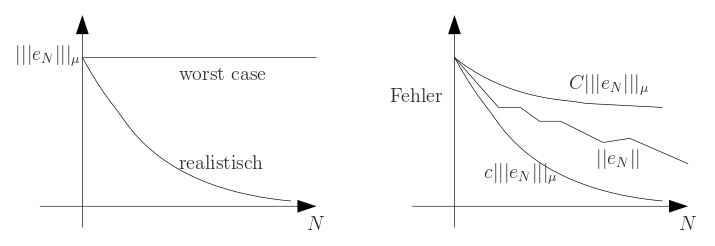
\includegraphics[width = 0.75 \textwidth]{Bilder/FehlerabfallEnergienorm.png}
		\caption{Fehlerabfall mit wachsender reduzierter Dimension.}{(aus B. Haasdonk, Reduzierte-Basis-Methoden, Skript zur Vorlesung SS 2011, Universität Stuttgart, IANS-Report 4/11, 2011.)}
		\label{fig:FehlerabfallEnergienorm}
	\end{figure}
\end{bem}

\begin{bem}[Gleichmäßige Konvergenz von Lagrange RB-Ansatz] \beginwithlistbem
	\begin{itemize}
		\item Sei $\p$ kompakt und $S_N := \set{\mu^1,\cdots,\mu^N} \subset \p$, $N \in \N$, sodass die sog.\ Füll-Distanz (fill-distance) $h_N$ gegen 0 geht:
			\begin{align*}
				h_N &:= \sup_{\mu \in \p} \dist(\mu, S_N), \quad \dist(\mu,S_N) := \min_{\mu' \in S_N} \norm{\mu - \mu'}\\
				\lim_{N \to \infty} h_N &= 0
			\end{align*}
		\item Falls $u(\mu)$, $u_N(\mu)$ Lipschitz-stetig mit Lipschitz-Konstante $L_u$ unabhängig von $N$, so folgt für alle $N$, $\mu$ und ``nächstes'' $\mu^* := \arg\min_{\mu' \in S_N} \norm{\mu-\mu'}$:
			\begin{align*}
				\norm{u(\mu)-u_N(\mu)} &\leq \norm{u(\mu)-u(\mu^*)} + \norm{u(\mu^*)-u_N(\mu^*)} + \norm{u_N(\mu^*)-u_N(\mu)}\\
				&\leq L_u \underbrace{\norm{\mu-\mu^*}}_{\leq h_N} + 0 + L_u \underbrace{\norm{\mu - \mu^*}}_{h_N} \leq 2 L_u h_N
			\end{align*}
		\item Also folgt uniforme Konvergenz
			\[
				\lim_{N \to \infty} \sup_{\mu \in \p} \norm{u(\mu)-u_N(\mu)} = 0
			\]
			\item Jedoch Konvergenzrate linear in $h_N$ ist nicht praktisch bedeutsam, weil $h_N$ sehr langsam mit $N$ abfällt, also muss $N$ sehr groß sein, um kleinen Fehler zu garantieren.
			\item Wir werden sehen, dass bei gleichmäßig koerziven Problemen und geschickter Wahl der $\mu^i$ sogar exponentielle Konvergenz erreicht wird.
	\end{itemize}
\end{bem}

\begin{lemma}[Fehler-Residuums-Beziehung] \label{3.12}
	Für $\mu \in \p$ definieren wir mittels der RB-Lösung $u_N$ das Residuum $r(\pdot;\mu) \in X'$ bzw.\ seinen Riesz-Repräsentanten $v_r(\mu) \in X$
	\[
		\dotp{v_r(\mu)}{v}_X := r(v;\mu) := f(v;\mu) - a(u_N(\mu),v;\mu) \quad \forall v \in X
	\]
	Dann erfüllt der Fehler $e(\mu) := u(\mu)-u_N(\mu)$
	\[
		a(e(\mu),v;\mu) = r(v;\mu) \quad \forall v \in X
	\]

	\begin{proof}
		$a(e(\mu),v;\mu) = \underbrace{a(u,v)}_{f(v)} - a(u_N,v) = r(v)$
	\end{proof}
\end{lemma}

\begin{bem} \beginwithlistbem
	\begin{itemize}
		\item Fehler erfüllt ``$\prob$ mit Residuum als rechte Seite''
		\item Insbesondere ist $r(v;\mu) = 0$ $\forall v \in X_N$ (wegen Galerkin-Orthogonalität)
		\item $r(\pdot;\mu) = 0 \quad \Rightarrow \quad e = 0$
	\end{itemize}
\end{bem}

\begin{satz}[A-posteriori Fehlerschätzer, absoluter Fehler] \label{3.13}
	Sei $\mu \in \p$, $u(\mu)$ bzw.\ $u_N(\mu)$ Lösung von $\prob$, $\rprob$ und $e=u-u_N$.
	Sei $\alpha_{LB}(\mu)$ eine untere Schranke für $\alpha(\mu)$ und $v_r \in X$ Riesz-Repräsentant von $r(\pdot;\mu)$ aus Lemma \ref{3.12}.
	Dann gelten folgende Schranken
	\begin{enumerate}
		\item Fehler in Energienorm
			\[
				\norm{e(\mu)}_\mu \leq \Delta_N^{en}(\mu) := \frac{\norm{v_r}}{\sqrt{\alpha_{LB}(\mu)}}
			\]
		\item Fehler in $X$-Norm $\norm\pdot$
			\[
				\norm{e(\mu)} \leq \Delta_N(\mu) := \frac{\norm{v_r}}{\alpha_{LB}(\mu)}
			\]
		\item Ausgabefehler
			\[
				|s(\mu)-s_N(\mu)| \leq \Delta_{N,s}(\mu) := \norm{l(\pdot;\mu)} \Delta_N(\mu)
			\]
	\end{enumerate}

	\begin{proof} \beginwithlistbew
		\begin{enumerate}
			\item Normäquivalenz \ref{2.5} impliziert
				\[
					\norm e \leq \frac{\norm{e}_\mu}{\sqrt{\alpha_{LB}(\mu)}}
				\]
				Damit folgt
				\[
					\norm{e}_\mu^2 = a_s(e,e) = a(e,e) = r(v) = \dotp{v_r}{e} \leq \norm{v_r} \norm{e} \leq \frac{\norm{v_r}}{\sqrt{\alpha_{LB}(\mu)}}
				\]
				Division durch $\norm{e}_\mu$ liefert die Behauptung i).
			\item Koerzivität liefert
				\[
					\alpha_{LB}(\mu) \norm{e}^2 \leq a(e,e) = r(e) = \dotp{v_r}{e} \leq \norm{v_r} \norm{e}
				\]
				Division durch $\alpha_{LB}$ und $\norm e$ liefert ii).
			\item Stetigkeit von $l$ liefert
				\[
					|s(\mu)-s_N(\mu)| = |l(u-u_N;\mu)| \leq \norm{l} \norm{u-u_N} \stackrel{ii)}{\leq} \norm{l} \Delta_N
				\]
		\end{enumerate}
	\end{proof}
\end{satz}

\begin{bem} \beginwithlistbem
	\begin{itemize}
		\item $\alpha_{LB}(\mu)$ soll eine \emph{schnell berechenbare} untere Schranke an $\alpha(\mu)$ sein, z.B.\ $\alpha_{LB}(\mu) := \bar \alpha$ falls $\bar \alpha$ bekannt, andere Möglichkeiten folgen später (``min $\Theta$'', ``SCM'').
		\item $\Delta_N$ ist also immer um Faktor $\sqrt{\alpha_{LB}(\mu)}$ schlechter.
		\item Beschränkung des Fehlers durch Residuums-Norm ist bekannte Technik aus FEM, um FEM-Lösung $u_h$ gegen Sobolev-Raum Lösung $u$ abzuschätzen.
			In diesem Fall ist $X$ $\infty$-dimensional und Residuums-Norm algorithmisch nicht berechenbar.
			In RB-Methoden wird $\norm{v_r}$ eine \emph{berechenbare} Größe sobald $X$ endlich-dimensional, z.B.\ FEM-Raum, ist.
			Für Residuum ist $u_N(\mu)$ erforderlich, daher sind Schranken ``\emph{a posteriori}''.
		\item Allgemeines Vorgehen (und alternative Begründung für ii)) zur Herleitung von Fehlerschranken: Zeige, dass Fehler $e$ erfüllt $\prob$ mit rechter Seite, genannt $r$ (Residuum), wende a-priori Stabilitätsaussage an:
			\[
				\norm{e} \leq \frac{\norm r}{\alpha(\mu)} \quad \text{z.B.\ Lax-Milgram}
			\]
			und erhalte berechenbare Größe durch Wahl $X=X_{FEM}$ und untere Schranke $\alpha_{LB}(\mu) \leq \alpha(\mu)$.
		\item Weil die Schranken beweisbare obere Schranken an Fehler darstellen, nennt man sie ``rigorose'' Fehlerschranken (vgl.\ ``zuverlässige'' Schätzer in FEM, bei denen jedoch die Konstante unbekannt ist).
		\item Fehlerschranken liefern eine Absicherung für RB-Methoden, ``certified'' RB-Methode, im Gegensatz zu vielen anderen Reduktionsmethoden (z.B.\ Krylov-Raum-Methoden).
		\item Ausgabefehler ist grob, indem $\Delta_N$ nur linear eingeht.
			Verbesserungen können für den ``compliant'' Fall oder mit primal-dual Techniken erreicht werden. ($\leadsto$ §\ref{sec-3.5})
	\end{itemize}
\end{bem}

\begin{kor}[Verschwindende Fehlerschranke] \label{3.14}
	Falls $u(\mu) = u_N(\mu)$ dann ist $\Delta_N(\mu) = \Delta_N^{en}(\mu) = \Delta_{N,s}(\mu) = 0$

	\begin{proof}
		\[
			0 = a(0,v;\mu) = a(e,v;\mu) = r(v;\mu)
		\]
		\[
			\Rightarrow r \equiv 0 \Rightarrow \norm{v_r} = 0 \Rightarrow \Delta_N = \Delta_N^{en} = \Delta_{N,s} = 0
		\]
	\end{proof}
\end{kor}

\begin{bem} \beginwithlistbem
	\begin{itemize}
		\item Dies ist initialer Wunsch an eine Fehlerschranke: diese soll verschwinden falls exakte Approximation vorliegt.
			Dies ist Grundlage dafür, dass der Faktor der Überschätzung endlich ist.
		\item Aussage ist trivial für \emph{effektive} Fehlerschätzer (sehen wir bald), aber in komplexen Problemen kann \ref{3.14} schon das maximal erreichbare sein.
		\item \ref{3.14} ist wieder sinnvoll um Programmcode zu validieren.
	\end{itemize}
\end{bem}

\begin{satz}[A-posteriori Fehlerschranken, relative Fehler]
	Mit Bezeichnungen/Voraussetzungen aus \ref{3.13} 
\end{satz}<++>
